\documentclass[10pt,twocolumn]{article}
% Rendered by make_paper.py from main.src.tex (do not edit main.tex; main.src.tex comes from md2tex.py).
\usepackage[margin=0.75in]{geometry}
\usepackage{graphicx,amssymb,hyperref,booktabs}
\usepackage[numbers]{natbib}
\usepackage{listings}\lstset{basicstyle=\ttfamily\scriptsize,breaklines=true,columns=fullflexible,keepspaces=true,frame=tb,framerule=0.3pt,aboveskip=4pt,belowskip=4pt,upquote=true}
\usepackage{style/shisso}
\shissorepo{github.com/ravediamond/paper-reward-models-stopping-rule}
\title{What a reward model can show depends on who stopped the episode: failure judges and monitors on a low-cost arm}
\date{}
\begin{document}
\twocolumn[\vspace*{0.32in}\shissopanel{What a reward model can show depends on who stopped the episode: failure judges and monitors on a low-cost arm}{Ravindu Somawansa\\[1pt]Shisso Robotics, Paris\\[1pt]\texttt{ravindu.somawansa@shissorobotics.com}}{Reward models that score robot rollouts are also used as failure detectors. We ask what such a detector has to beat on a dataset where operators stop the episodes. We use two SO-101 datasets. ArmnetBench has {{ab_n}} rollouts and no time limit: its operators stop a success when the task is done and let a failure run on. There, episode length alone separates failure from success at AUROC {{len_within}} within policy, and the better of two zero-shot reward models reaches {{rbm_within}}. On our own {{own_n}} rollouts the operator stopped each run by judgment, and length falls to {{own_len}}, close to chance. A judge that sees the finished episode reaches AUROC {{flora_auc}} on 50 of them. The baseline a detector has to beat depends on how the dataset's episodes were stopped.}{\textbf{Code and rows:} \texttt{github.com/ravediamond/paper-reward-models-stopping-rule}\quad\textbf{Reproduce:} \texttt{make check}}\vspace{4pt}]
\section{Introduction}
Papers that evaluate a reward model as a failure detector normally compare it with other learned detectors. On ArmnetBench the operator stopped each rollout and there was no set time limit. Successes are cut at completion and failures run on, and the length of an episode also encodes its outcome. The identity of the policy that ran can carry it too, and we call this the policy-identity null (mainly with models that give out-of-distribution results). On our own rollouts the operator stopped each run by his judgment, and both signals are weaker. The way a dataset ends its episodes is its stopping rule. None of the reward-model papers in our library reports the stopping rule or a length baseline.

We started with a narrower claim, that elapsed time is the reward model to beat. Our own rollouts did not support it. Length is near chance on them. A robot-trained judge passed its threshold on them. What differs between the two results is how the episodes ended, so the stopping rule became the subject of the paper.

The question of this paper is what a reward model has to beat to count as a failure detector on a dataset where operators stop the episodes. We measured length on ArmnetBench \citep{armnetbench} and on our own rollouts, and compared it with two zero-shot reward models, Robometer \citep{robometer} and TOPReward \citep{topreward}. On our {{own_n}} operator-stopped rollouts we also compared it with every judge and monitor we had run. Every bar and every primary score was fixed before the test it judges.

\begin{figure*}[t]\centering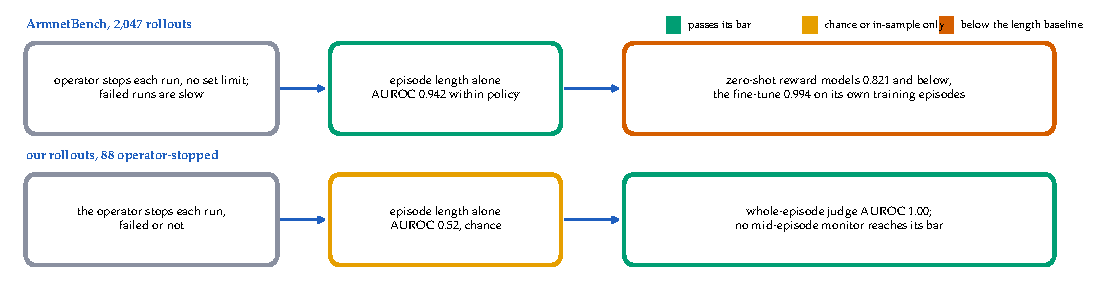
\includegraphics[width=\textwidth]{fig/stopping_rule.pdf}\caption{\textbf{What the baseline is depends on how the episodes ended.} ArmnetBench (operator-stopped, no set limit): length {{len_within}} within policy, both zero-shot reward models below it, the fine-tune only in-sample. Our operator-stopped rollouts: length {{own_len}}, chance; a whole-episode judge {{flora_auc}}; no mid-episode monitor reaches its bar.}\end{figure*}


\section{Data and labels}
ArmnetBench v0.1 \citep{armnetbench} has 8 tasks and {{n_pol}} policies on the SO-101. We use its {{ab_n}} policy rollouts that have a success or failure class ({{ab_ok}} successes, {{ab_fail}} failures) and leave out the teleoperated episodes. Robometer scored {{rbm_n_scored}} rollouts, the extra ones labelled suboptimal; every AUROC here uses the {{ab_n}}. The benchmark sets no time limit. Its operators stop a success when the task is done and let a failure run on, so only {{hit_fail}} \% of failures reach the longest episode of their task. One task, pushing a Displayport cable ({{dp_n}} rollouts), has rollouts of a single class, so it has no per-task AUROC.

Our own data are {{own_n}} labelled episodes of one task, placing one bowl in another, on one SO-101 arm with a Jetson Orin NX. TOPReward scored {{topr_own_n}} of them, with {{own_fail}} failures, {{own_turbo_fail}} of which come from one policy, TurboVLA \citep{turbovla}. Every judge and monitor used the {{topr_own_nt_n}} of these {{topr_own_n}} that TurboVLA did not run (42 successes, 8 failures). The author was the operator, stopped each run and labelled it at rest, and was not blind to the policy. What these data cannot show: the judge and monitor results rest on 8 failures of one task, and the judges' operating thresholds were chosen on the same 50 episodes.

\section{The length baseline}
The goal of a failure detector is to rank failed episodes above successful ones, and we report its failure AUROC (0.5 is chance, 1 is perfect). Pooled means all rollouts taken as one set. A pooled AUROC can be high only because some policies fail more often than others, so we also report it within policy: the AUROC inside each policy's rollouts, averaged with each policy weighted by its number of success--failure pairs (pair-weighted; the code is in the appendix). The free baseline is episode length, with longer meaning failure. It is strong on ArmnetBench because of the stopping rule: a success is stopped when it is done and a failure runs on. Intervals are 95 \% bootstrap intervals over episodes (2,000 resamples). When a paired interval on a difference lies entirely below zero, the loss is not luck.

On ArmnetBench, episode length is a strong failure detector within each policy (Table 1, Fig. 2). Pooled over policies
it reaches {{len_pooled}}. Within each policy it ranges from {{len_pol_min}} to {{len_pol_max}}. Pair-weighted, the
within-policy value is {{len_within}}, with a CI of {{len_within_lo}}--{{len_within_hi}}.

We ran Robometer-4B \citep{robometer} zero-shot, as its authors ship it (the authors' method). It scores {{rbm_pooled}} pooled and {{rbm_within}}
within policy (CI {{rbm_w_lo}}--{{rbm_w_hi}}). Its paired difference to length within policy has a 95 \% CI of {{rbm_d_lo}} to {{rbm_d_hi}}, entirely below zero. We ran TOPReward \citep{topreward} with Qwen3-VL-8B \citep{qwen3vl} and no training. Its paper does not give the number of prefixes, the frames per query or the wording of the Yes/No question, so we chose them, and we count it as the authors' method fitted to our data. It scores {{topr_within}} within
policy. Its paired difference to length has a 95 \% CI of {{topr_d_lo}} to {{topr_d_hi}}. The primary score is the success probability for Robometer and the success score of its paper for TOPReward. Two other scores from the same runs are in Table 1 as descriptive rows. They are higher,
and still below length.


\begin{table}[t]\centering\scriptsize
\setlength{\tabcolsep}{3pt}\renewcommand{\arraystretch}{1.1}
\begin{tabular}{>{\raggedright\arraybackslash}p{2.3cm}>{\raggedright\arraybackslash}p{1.5cm}>{\raggedright\arraybackslash}p{2.0cm}>{\raggedright\arraybackslash}p{2.1cm}}
\toprule
\shissohead signal & method as & pooled & within policy \\
\midrule
episode length & free baseline & {{len_pooled}} ({{len_pooled_lo}}--{{len_pooled_hi}}) & {{len_within}} ({{len_within_lo}}--{{len_within_hi}}) \\
length seen up to 50 \% of the longest run & free baseline & --- & {{t50_within}} ({{t50_lo}}--{{t50_hi}}) \\
Robometer-4B, success probability & authors', as shipped & {{rbm_pooled}} ({{rbm_lo}}--{{rbm_hi}}) & {{rbm_within}} ({{rbm_w_lo}}--{{rbm_w_hi}}) \\
Robometer-4B, last progress (descriptive) & authors', as shipped & {{rbm_prog}} (no CI) & --- \\
Robometer-4B fine-tuned on ArmnetBench, success probability (in-sample) & released fine-tune & {{ft_pooled}} ({{ft_lo}}--{{ft_hi}}) & {{ft_within}} ({{ft_w_lo}}--{{ft_w_hi}}) \\
TOPReward, success score & authors', fitted & {{topr_pooled}} ({{topr_pooled_lo}}--{{topr_pooled_hi}}) & {{topr_within}} ({{topr_lo}}--{{topr_hi}}) \\
TOPReward, Yes/\allowbreak{}No component (descriptive) & authors', fitted & --- & {{topr_yn_within}} \\
\bottomrule
\end{tabular}
\caption{ArmnetBench, failure AUROC with 95 \% episode-bootstrap CIs, on the {{ab_n}} rollouts. Pooled: all rollouts as one set; within policy: pair-weighted mean of the per-policy AUROCs. Read down the within-policy column: no zero-shot reward-model score reaches length, and the fine-tune row is in-sample.}
\end{table}


\begin{figure}[t]\centering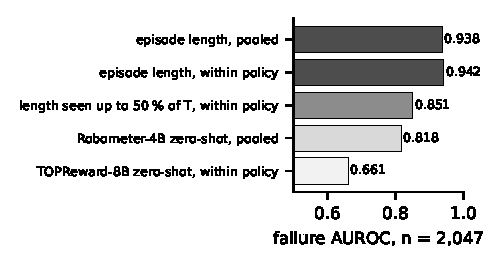
\includegraphics[width=\columnwidth]{fig/armnetbench.pdf}\caption{Failure AUROC on ArmnetBench: episode length against two zero-shot reward models. Length leads both, pooled and within policy (95 \% CIs where available).}\end{figure}


We also scored the released ArmnetBench fine-tune of Robometer, \texttt{jesbu1/robometer-4b-fft-armnet-tiled}, since the obvious reply to a zero-shot result is to use it. Its model card lists a dataset of all {{ft_train_n}} ArmnetBench episodes, with no held-out split, as its training data. Every episode we score was therefore a training episode with its label, and the result is in-sample. On the {{ft_n}} rollouts it scores {{ft_pooled}} pooled and {{ft_within}} within policy, {{ft_d}} above length (paired CI {{ft_d_lo}} to {{ft_d_hi}}). This shows that the labels can be fit. It does not show that a reward model beats length on rollouts it has not seen. We gave it 8 frames spread over the 64 of each tiled video, the length it was trained on. Scoring all 64 frames on {{ft_sub_n}} episodes gives {{ft_sub64}} pooled against {{ft_sub8}} for 8 frames.

\section{Length is more than the longest episode}
Only {{hit_fail}} \% of failures run as long as the task's longest episode, which we use as a reference length (the benchmark sets no time limit). At half that length, {{t50_run_fail}} \% of failures are still running, and only {{t50_run_ok}} \% of successes are. Length observed up to that cut gives {{t50_within}} within policy (Fig. 3). The CI is {{t50_lo}}--{{t50_hi}}. TOPReward on frames up to the same cut reaches {{topr_cap}}. Robometer's success probability at the last frame before the cut gives {{rbm_t50}} within policy (CI {{rbm_t50_lo}}--{{rbm_t50_hi}}), which is below length at that cut. At a quarter of the longest episode the order is the other way, {{rbm_t25}} for Robometer against {{len_t25}} for length, and by three quarters length is ahead again, {{len_t75}} against {{rbm_t75}}. These are prefixes of one pass over the whole episode (§7). Failed rollouts are slow; most do not reach the task's longest episode.

\begin{figure}[t]\centering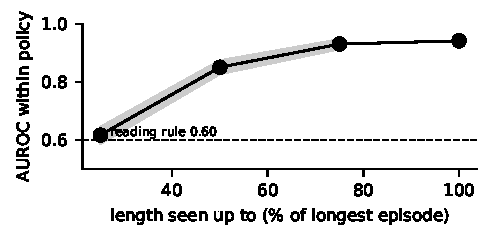
\includegraphics[width=\columnwidth]{fig/truncation.pdf}\caption{Length observed up to a fraction of the task's longest episode, AUROC within policy: most of the signal is there by half the episode (band: 95 \% CI).}\end{figure}


\begin{shissofinding}[Own rollouts.]
On our own operator-stopped rollouts, length is at chance. It gives {{topr_own_len}} on the {{topr_own_n}} rollouts TOPReward scored and {{own_len}} on all {{own_n}}. Here the policy-identity null is the baseline to beat: it scores each episode by the failure rate of the policy that ran it, on the same episodes. It is strong because {{own_turbo_fail}} of the {{own_fail}} failures in the {{topr_own_n}} come from one policy, TurboVLA \citep{turbovla}. Neither reward model beats policy identity. TOPReward scores {{topr_own}} (CI {{topr_own_lo}}--{{topr_own_hi}}), and policy identity alone {{topr_own_pol}}. On the {{topr_own_nt_n}} episodes without TurboVLA, TOPReward scores {{topr_own_nt}}. Robometer scores {{own_rbm}} on all {{own_n}}, and policy identity {{own_rbm_pol}}.
\end{shissofinding}

\section{Judges and monitors on our rollouts}
A judge looks at the finished episode and says whether it succeeded. A monitor reads the episode while it runs and must raise an alarm before the end, early enough for the robot to stop. Table 2 gives each a threshold-free AUROC where one is defined, and the failures caught and successes flagged at its operating point, the score threshold that turns scores into flags. For the judges that point was chosen on the same 50 episodes (in-sample), so their counts are optimistic. The monitors' thresholds were fixed before scoring.

We first ran a deterministic top-camera check, with colour masks and geometry and no learning. It is right on {{g9c3_acc}} \% of judged episodes. It has {{g9c3_fp}} false positives and {{g9c3_fn}} false negatives. The Wilson interval on the false positives is {{g9c3_fp_ci}}. We
then gave Flora-Rewarder-27B \citep{flora27b} a 64-frame two-view clip and NVIDIA's prompt. Its threshold-free AUROC is {{flora_auc}}. The bootstrap CI is {{flora_lo}}--{{flora_hi}}. At its in-sample operating point it flags {{flora_f}} of 8 failures at {{flora_s}} of 42 successes. The Wilson interval on those false alarms is {{flora_s_ci}}. The bar was
at least 6 of 8 failures at no more than 2 of 42 successes, so it passes. Its base model, Qwen3.5-27B \citep{qwen35}, has
no robot fine-tune. On the same input it also passes, with AUROC {{q27_auc}} and {{q27_f}} of 8 at {{q27_s}} of 42. The interval on that AUROC is {{q27_lo}}--{{q27_hi}}. The input format mattered more than the fine-tune. Qwen3.5-9B \citep{qwen35} flags {{q9_s}} successes
and fails. Gemini 3.8 Flash \citep{gemini38} fails by one false alarm.

The bar for mid-episode monitors is at least 5 of 8 failures at no more than 1 of 20 false interventions. No monitor reaches it on these 50 rollouts (Fig. 4). The surprise of a separate world model, trained in the LeWorldModel recipe \citep{lewm}, catches {{w1_l2}} of 8 at {{w1_l2_fi}} of 42. Its AUROC is {{w1_l2_auc}}. A Gemini sliding-window judge catches {{tau_caught}}. The first action-conditioned risk head on the world model's latent reached AUROC {{r1_log_auc}}. It read elapsed time, so we withdrew that result. We built a second version without time or length. It catches {{r2_log_c}} of 8 at {{r2_log_fi}} of 42. Its AUROC is {{r2_log_auc}}, and {{r2_sh_auc}} with shuffled actions. The MLP variant catches {{r2_mlp_c}} of 8 and flags {{r2_mlp_fi}} of 42.

Two comparisons were added after these tests and are exploratory, with no bar. On the 50 episodes the free baselines are weaker than on the {{topr_own_n}}, because TurboVLA did not run any of them: policy identity gives {{s50_pol}} and length {{s50_len}}. Flora's AUROC is {{s50_fl_d}} above policy identity, with a paired CI of {{s50_fl_lo}} to {{s50_fl_hi}}, entirely above zero; for Qwen3.5-27B the interval, {{s50_q_lo}} to {{s50_q_hi}}, contains zero. The risk head is our own design after ReAP \citep{reap}. ReAP releases no code, so we also rebuilt its Stage 1 detector and Stage 2 predictor from the paper, with a smaller DINOv2, one camera, training data mostly from other tasks (ArmnetBench) and one seed of the five planned. It catches {{reap_caught}} of 8 at {{reap_fi}} of 42, AUROC {{reap_auroc}}, and fails the monitor bar. On our side: 8 failures, one task, one seed and a smaller backbone than the paper's.


\begin{table*}[t]\centering\scriptsize
\setlength{\tabcolsep}{3pt}\renewcommand{\arraystretch}{1.1}
\begin{tabular}{p{2.8cm}p{2.2cm}p{1.0cm}p{3.1cm}p{1.1cm}p{1.2cm}p{2.3cm}}
\toprule
\shissohead method & method as & kind & AUROC & caught / 8 & flagged / 42 & threshold \\
\midrule
policy identity & free baseline & at rest & {{s50_pol}} & --- & --- & --- \\
episode length & free baseline & at rest & {{s50_len}} & --- & --- & --- \\
colour judge (no learning) & ours & at rest & --- ({{g9c3_acc}} \% right, {{g9c3_fp}} FP, {{g9c3_fn}} FN) & --- & --- & fixed rule \\
Flora-Rewarder-27B & authors' prompt & at rest & {{flora_auc}} ({{flora_lo}}--{{flora_hi}}) & {{flora_f}} & {{flora_s}} & in-sample \\
Qwen3.5-27B, same input & base model & at rest & {{q27_auc}} ({{q27_lo}}--{{q27_hi}}) & {{q27_f}} & {{q27_s}} & in-sample \\
Qwen3.5-9B, same input & base model & at rest & {{q9_auc}} & {{q9_f}} & {{q9_s}} & in-sample \\
Gemini 3.8 Flash, same input & base model & at rest & {{gem_auc}} & {{gem_f}} & {{gem_s}} & in-sample \\
Gemini sliding windows & ours & monitor & --- & {{tau_caught}} & {{tau_fi}} & fixed before scoring \\
world-model surprise & ours, LeWorldModel recipe & monitor & {{w1_l2_auc}} & {{w1_l2}} & {{w1_l2_fi}} & fixed before scoring \\
world-model latent drift & ours, LeWorldModel recipe & monitor & {{w1_cos_auc}} & {{w1_cos}} & {{w1_cos_fi}} & fixed before scoring \\
risk head, logistic (v2) & ours, after ReAP & monitor & {{r2_log_auc}} & {{r2_log_c}} & {{r2_log_fi}} & 5-fold by episode \\
risk head, MLP (v2) & ours, after ReAP & monitor & --- & {{r2_mlp_c}} & {{r2_mlp_fi}} & 5-fold by episode \\
ReAP Stage 1 + 2, rebuilt & authors', reduced & monitor & {{reap_auroc}} & {{reap_caught}} & {{reap_fi}} & one global threshold \\
\bottomrule
\end{tabular}
\caption{Judges and monitors on the 50 operator-stopped rollouts (42 successes, 8 failures). Judges see the finished episode; monitors are held to $\geq$ 5/8 caught at $\leq$ 1/20 false interventions. "Method as": whose method ran; the free baselines and the ReAP rebuild were added after the tests (exploratory).}
\end{table*}


\begin{figure}[t]\centering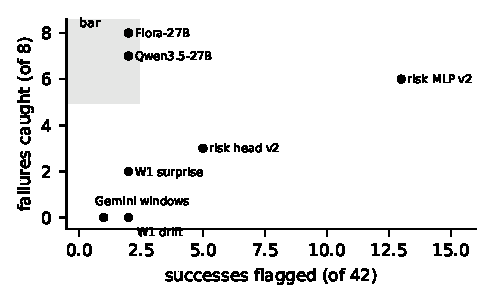
\includegraphics[width=\columnwidth]{fig/own_monitors.pdf}\caption{Failures caught against successes flagged on the 50 rollouts. No monitor (circles) reaches its shaded bar; the judges at rest (squares) sit at their in-sample operating point, where the monitor bar does not apply.}\end{figure}


\section{Related work}
Robometer \citep{robometer} scales a general-purpose reward model through trajectory comparisons. TOPReward \citep{topreward} reads the token probabilities of a video-language model as hidden rewards. A survey of verifiers for robot policies \citep{nofreechecker} covers the wider family. FAIL-Detect \citep{faildetect} and SAFE \citep{safe} learn uncertainty- and feature-based failure scores for imitation and VLA policies. FARM \citep{farm} reads failure signals from the internal states of a frozen world model, like our world-model monitors. Our risk head follows ReAP \citep{reap}, which predicts action-conditioned risk. VLA-Corrector \citep{vlacorrector} verifies stages, Spotter \citep{spotter} adds a reflecting VLM, and REMORA \citep{remora} tracks progress through errors and recovery. ArmnetBench \citep{armnetbench} and a standardized SO-101 VLA benchmark \citep{so101bench} evaluate policies on the same arm. We found no report of the elapsed-length baseline under the dataset's stopping rule in any of them.

\section{Limitations}
The judge pass on our own rollouts rests on 8 failures. Its operating thresholds were chosen on the same 50 episodes.
A single operator, the author, labelled them and was not blind to the policy. The threshold-free AUROCs do not depend
on the threshold. Fresh rollouts scored at the same thresholds would confirm the operating points.
{{own_turbo_fail}} of the {{own_fail}} failures in our {{topr_own_n}} rollouts are TurboVLA's. Any score that reads the policy
therefore gets the policy-identity null for free. The risk head is trained and tested on the same 50 episodes. Five
folds by episode keep episodes from leaking, but tasks and policies leak. The fine-tune comparison is in-sample, because the release has no held-out episodes, and its config needed three training-only keys removed to load in the pinned code. Robometer's truncated scores are prefixes of one pass over the whole episode. A frame's value may depend on later frames, so a pass over a clip that ends at the cut could give a different number. The {{rbm_n_rescore}} episodes that ran out of memory in the first pass were scored in a second pass on a larger GPU, with every frame kept. TOPReward's paper does
not give its prefix count, frames per query or Yes/No wording, so those are our choices. The ArmnetBench result covers
eight tasks. The reference length is each task's longest episode; the benchmark sets no time limit.

\section{Conclusion}
\begin{shissofinding}[Conclusion.]
On ArmnetBench, where the operator stopped each rollout and there was no set time limit, episode length beat both zero-shot reward models, and a fine-tune beat it only on the episodes it was trained on. On our operator-stopped rollouts length was at chance, and a judge that saw the whole finished episode caught the failures. When you evaluate a reward model as a failure detector, report episode length within policy on the same rows and say how the episodes ended.
\end{shissofinding}
\bibliographystyle{plainnat}
\bibliography{refs}

\appendix
\section*{Appendix: the within-policy AUROC}
The within-policy value pair-weights the per-policy AUROCs (\texttt{repro/length-null/scripts/length\_analysis.py}):

\begin{lstlisting}
def stratified(df, score, by="policy_type"):
    """Pair-weighted mean of per-stratum AUROCs (weights successes x failures)."""
    num = den = 0.0
    for _, g in df.groupby(by):
        a = auroc(g.y, g[score]); w = g.y.sum() * (~g.y).sum()
        if a is not None:
            num += a * w; den += w
    return num / den if den else None
\end{lstlisting}

The code, the expected result files and the protocol of every analysis are in the repository; its README maps each analysis to its files.
\end{document}
